\section{Results}

Execution+mypy repair substantially outperforms execution-only repair on
HumanEval+ (+8.94pp pass@1), consistently across three seeds. The improvement
is not explained by type-targeted correction.

\subsection{RQ1: Mypy Signal Existence (h-e1)}

Figure~\ref{fig:mypy_fraction} shows the mypy error rate in GPT-4o-mini's
failing solutions by benchmark. On HumanEval+, \textbf{70\% of failing
solutions} (21/30 failing) have at least one mypy error --- substantially
exceeding the 10\% existence gate. On MBPP+, \textbf{0\% of failing solutions}
(0/21 failing) have mypy errors.

\begin{figure}[h]
\centering
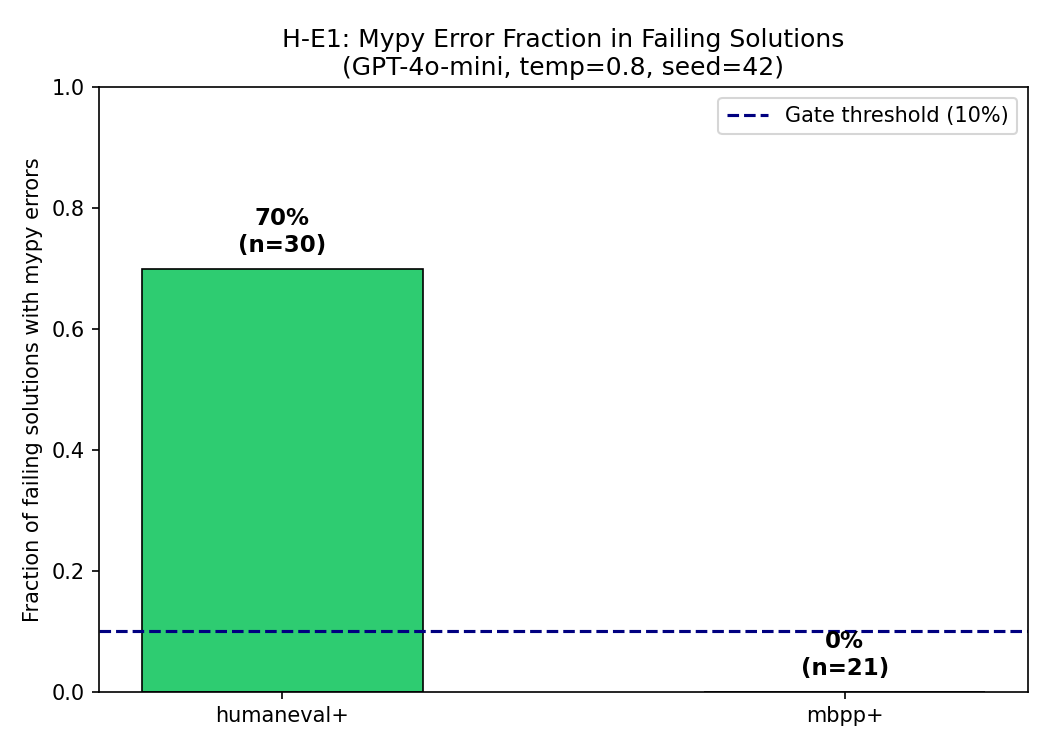
\includegraphics[width=0.9\columnwidth]{figures/fig1_mypy_fraction_by_benchmark.png}
\caption{Fraction of failing solutions with mypy-detectable errors on
HumanEval+ and MBPP+.}
\label{fig:mypy_fraction}
\end{figure}

This benchmark divergence is complete and unexpected. All 100\% of detected
mypy errors are in the \texttt{name-defined} category --- hallucinated function
or variable names (Figure~\ref{fig:error_category}).

\begin{figure}[h]
\centering
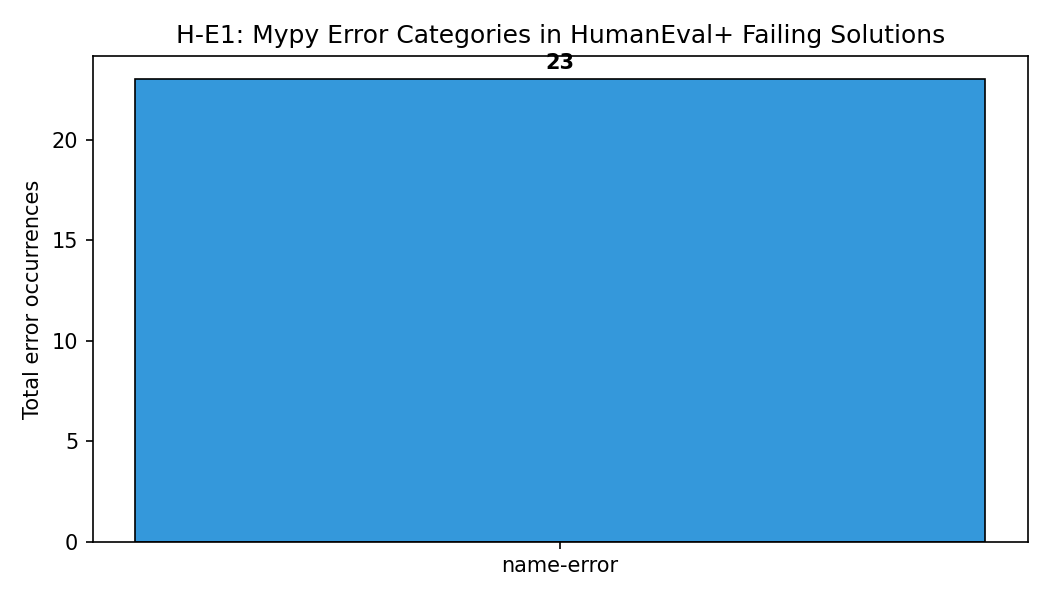
\includegraphics[width=0.9\columnwidth]{figures/fig2_error_category_breakdown.png}
\caption{mypy error category breakdown in HumanEval+ failing solutions.}
\label{fig:error_category}
\end{figure}

\emph{Interpretation:} The mypy signal exists on HumanEval+ at sufficient
density (70\%) to drive repair improvement. The 0\% rate on MBPP+ predicts no
mypy benefit there --- removing MBPP+ from the primary pass@1 comparison.

\subsection{RQ2: LLM Consumption of mypy Feedback (h-m1)}

Among 20 HumanEval+ problems with $\geq$1 initial mypy error (Condition B),
mean mypy errors follow a near-perfect monotonic decrease: \textbf{1.55 at
round 1 $\to$ 0.00 by round 2}, remaining at 0.00 through rounds 3--5.

\begin{figure}[h]
\centering
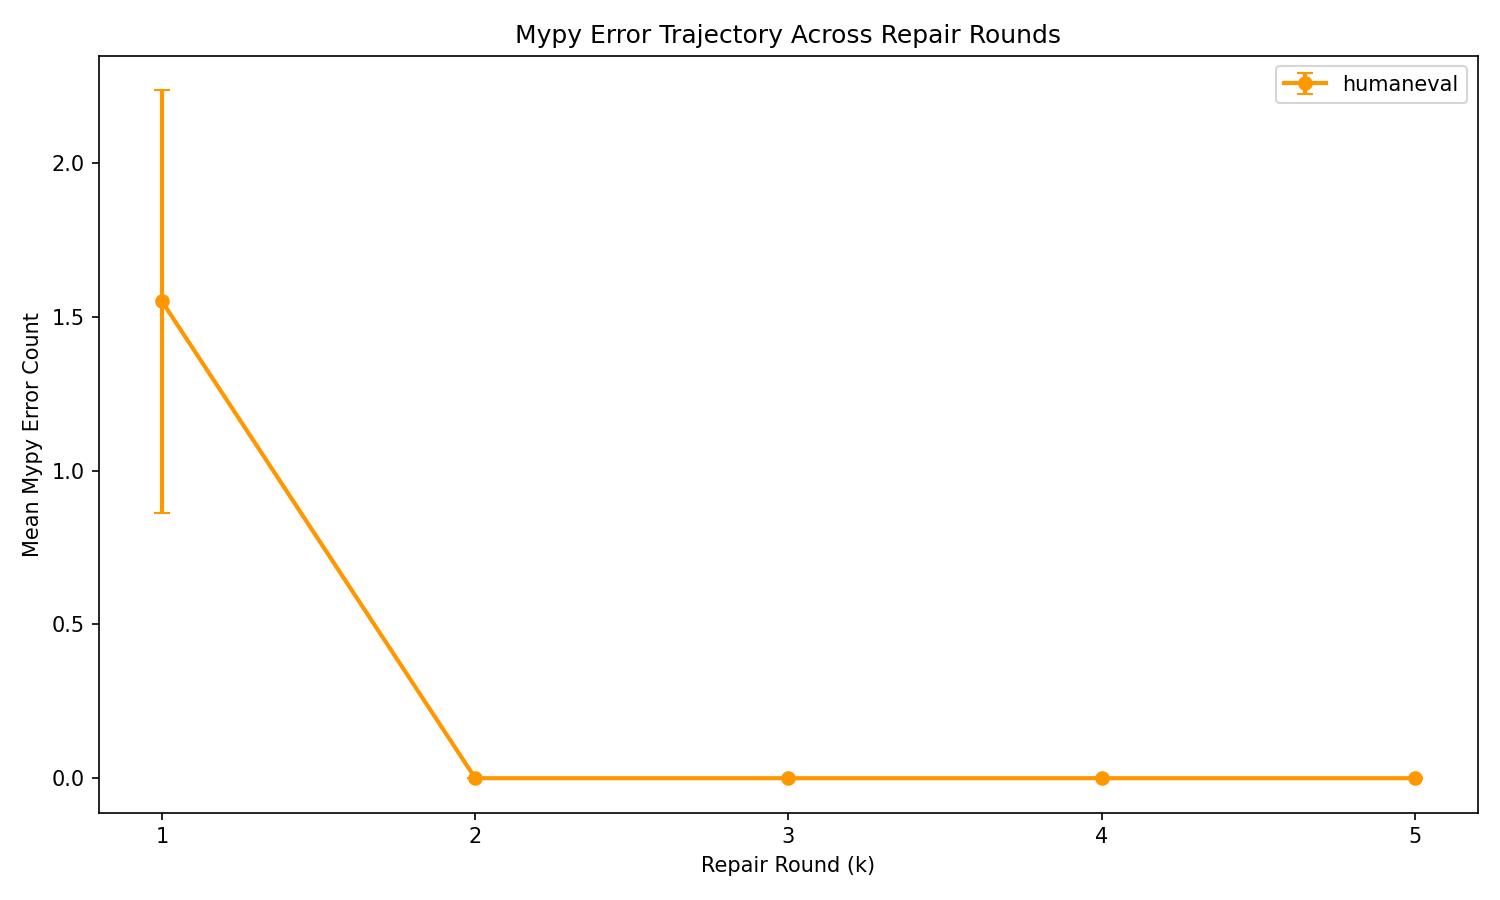
\includegraphics[width=0.9\columnwidth]{figures/error_trajectory.png}
\caption{Mean mypy error count by repair round ($n$=20 problems with $\geq$1
initial error). Spearman $\rho = -0.707$.}
\label{fig:error_trajectory}
\end{figure}

\emph{Interpretation:} GPT-4o-mini at temperature=0.0 eliminates all detected
mypy errors in a single repair round, with no backsliding. The LLM is an
effective consumer of structured static analysis output. Rapid saturation
confirms that $k$=5 is more than sufficient.

\subsection{RQ3: Type-Specificity of Improvement (h-m2)}

\begin{table}[h]
\centering
\caption{Repair rates by problem type and condition (HumanEval+, $n$=22
type-error problems, $n$=142 non-type-error problems, seed=42, $k$=5).}
\label{tab:type_specificity}
\begin{tabular}{@{}llll@{}}
\toprule
Problem type & Cond.\ A & Cond.\ B & Delta \\
\midrule
Type-error ($n$=22) & 90.9\% & 90.9\% & \textbf{0.000} \\
Non-type-error ($n$=142) & ${\sim}$78\% & ${\sim}$79\% & +0.6\% \\
\bottomrule
\end{tabular}
\end{table}

Type-specificity differential = $0.000 - 0.006 = \mathbf{-0.006}$. Both
conditions achieve exactly 90.9\% repair rate on type-error problems.

\begin{figure}[h]
\centering
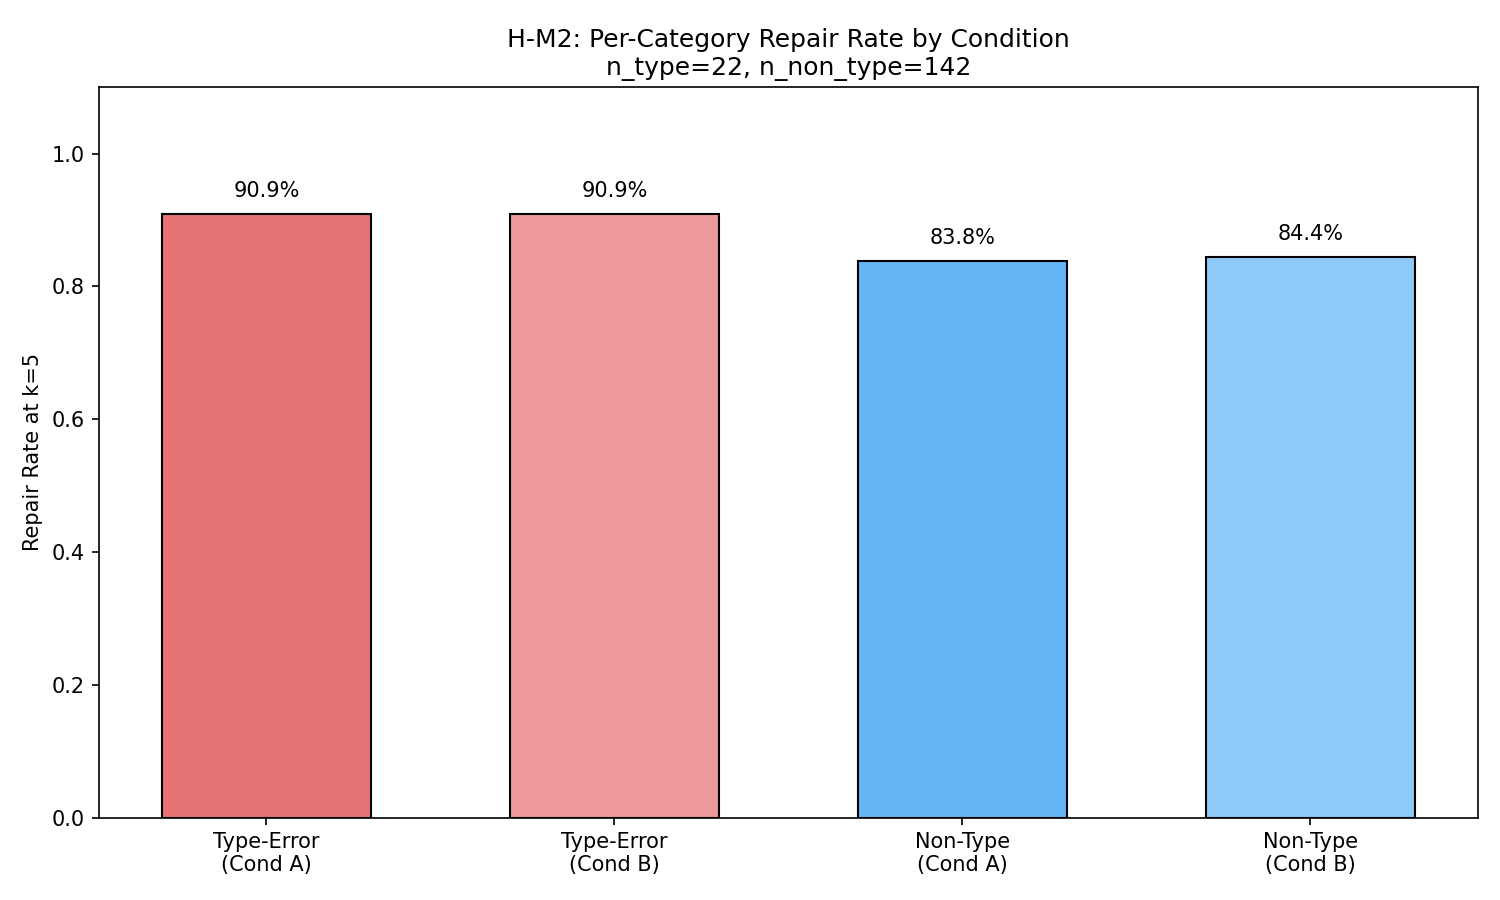
\includegraphics[width=0.9\columnwidth]{figures/repair_rate_comparison.png}
\caption{Repair rates for type-error and non-type-error problems under
Conditions A and B.}
\label{fig:repair_rate}
\end{figure}

\begin{figure}[h]
\centering
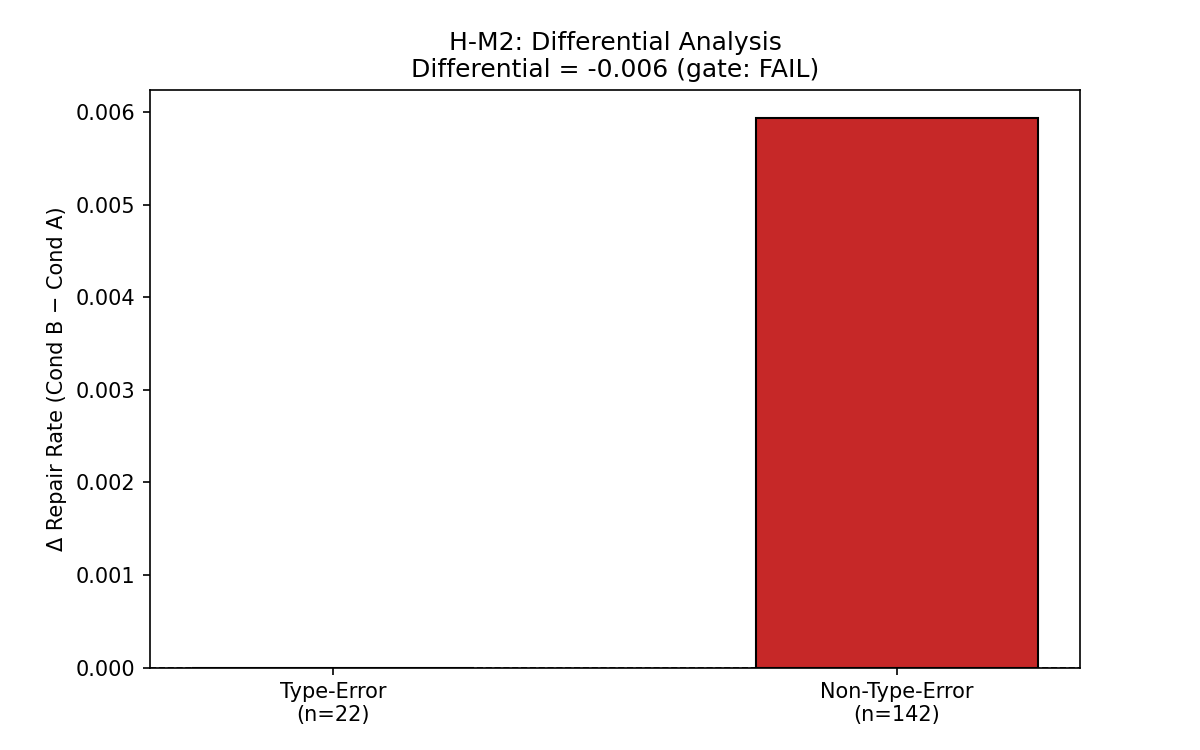
\includegraphics[width=0.9\columnwidth]{figures/differential_chart.png}
\caption{Type-specificity differential chart.}
\label{fig:differential}
\end{figure}

\emph{Interpretation:} The type-specificity mechanism is not active at $k$=5
saturation. Type-error problems reach a 90.9\% ceiling under execution-only
repair; mypy adds no further improvement for these problems. The overall
improvement must arise from a different mechanism --- most plausibly general
context enrichment.

\subsection{RQ4: Overall Pass@1 Comparison (h-m3)}

\begin{table}[h]
\centering
\caption{pass@1 on HumanEval+ (164 problems, GPT-4o-mini, $k$=5 rounds).}
\label{tab:pass1}
\begin{tabular}{@{}llll@{}}
\toprule
Seed & Cond.\ A & Cond.\ B & Delta \\
\midrule
42 & 79.9\% & 86.6\% & +6.7pp \\
123 & 76.8\% & 87.8\% & +11.0pp \\
456 & 78.1\% & 87.2\% & +9.2pp \\
\midrule
\textbf{Mean} & \textbf{78.25\%} & \textbf{87.20\%} & \textbf{+8.94pp} \\
\bottomrule
\end{tabular}
\end{table}

Execution+mypy repair achieves \textbf{87.20\% pass@1} versus \textbf{78.25\%}
for execution-only --- a \textbf{+8.94pp} improvement (seed std: A = $\pm$1.56pp,
B = $\pm$0.49pp; delta range: 6.7pp to 11.0pp). The direction is consistent
across all three seeds (no seed shows A $\geq$ B).

\emph{Interpretation:} This is the primary empirical contribution. The
improvement is real, reproducible, and substantial. Combined with the RQ3 null
result, this establishes that mypy improves repair quality broadly --- through
general diagnostic context enrichment rather than type-targeted correction.

\subsection{RQ5: Z3 Counterexample Feedback (h-z1)}

Figure~\ref{fig:z3_funnel} shows the Z3 pipeline funnel.

\begin{figure}[h]
\centering
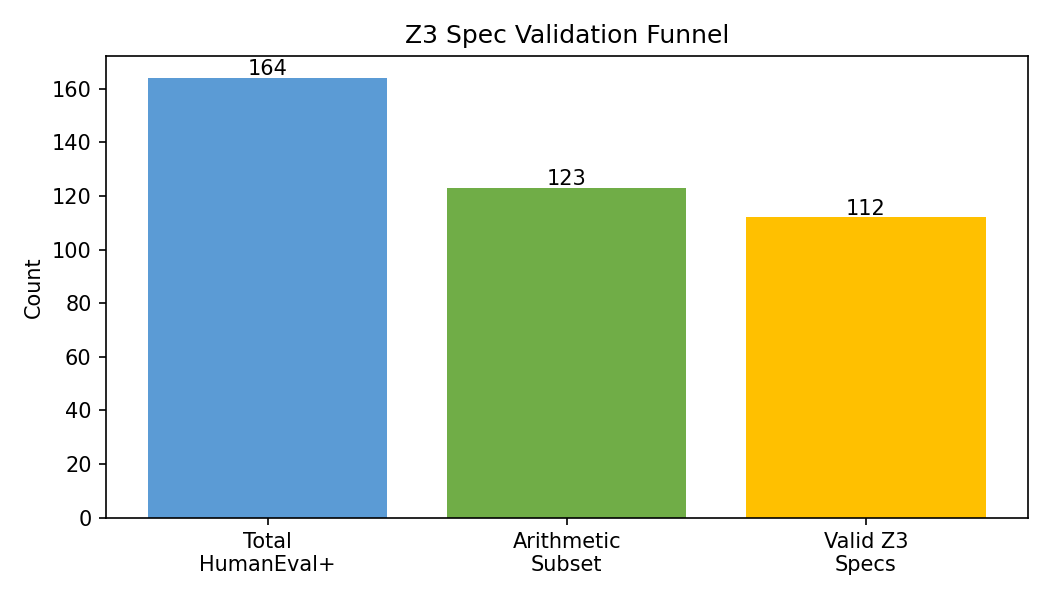
\includegraphics[width=0.9\columnwidth]{figures/z3_funnel.png}
\caption{Z3 validation funnel: 123 arithmetic problems $\to$ 112 valid specs
(91.1\%) $\to$ 18 problems with $\geq$1 counterexample (16.1\% CE rate).}
\label{fig:z3_funnel}
\end{figure}

\begin{figure}[h]
\centering
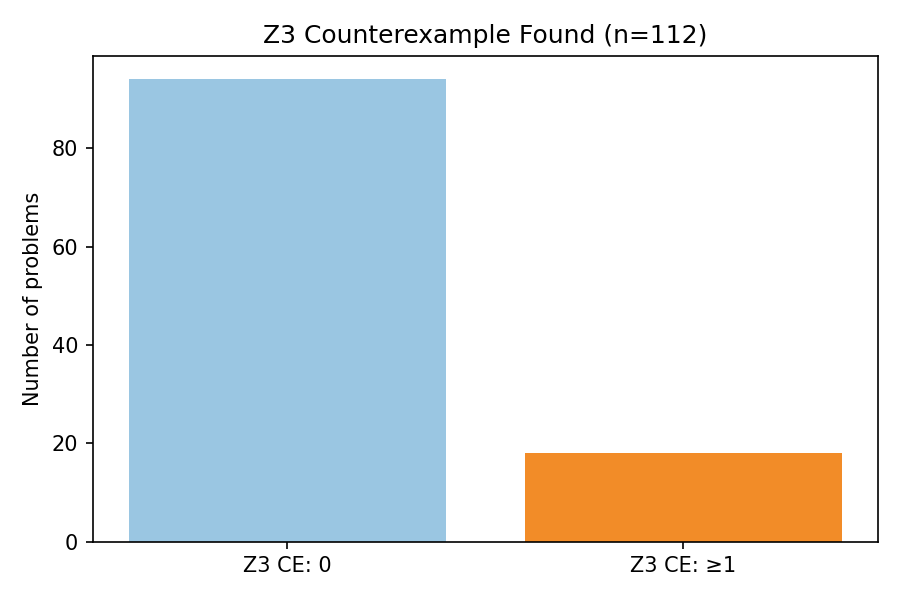
\includegraphics[width=0.9\columnwidth]{figures/z3_ce_distribution.png}
\caption{Z3 counterexample found vs.\ not found by problem.}
\label{fig:z3_ce}
\end{figure}

\begin{table}[h]
\centering
\caption{pass@1 on arithmetic subset ($n$=112, valid Z3 specs, seed=42, $k$=5).}
\label{tab:z3}
\begin{tabular}{@{}ll@{}}
\toprule
Condition & pass@1 \\
\midrule
B (execution+mypy) & 86.6\% \\
C (execution+mypy+Z3) & 85.7\% \\
Delta (C $-$ B) & \textbf{$-$0.9pp} \\
\bottomrule
\end{tabular}
\end{table}

\begin{figure}[h]
\centering
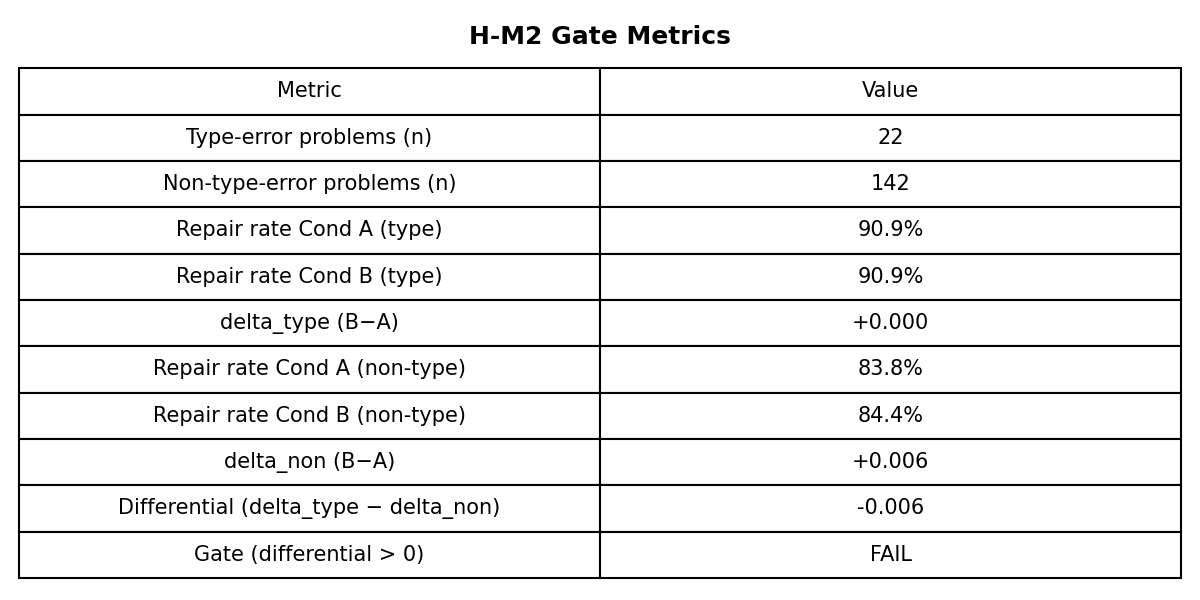
\includegraphics[width=0.9\columnwidth]{figures/gate_metrics.png}
\caption{pass@1 comparison between Conditions B and C on the arithmetic subset.}
\label{fig:gate_metrics}
\end{figure}

\emph{Interpretation:} Z3 CE feedback does not improve pass@1 beyond
execution+mypy. Two factors explain this: CE activation rate is low (16.1\%)
and base pass@1 (86.6\%) leaves only 13.4\% headroom. The Z3 pipeline's
primary contribution is the 91.1\% spec validity rate, establishing feasibility
for future work on harder problems with more headroom.

\subsection{Summary}

\begin{table}[h]
\centering
\caption{Summary of sub-hypothesis outcomes.}
\label{tab:summary}
\begin{tabular}{@{}lllll@{}}
\toprule
RQ & Hyp. & Finding & Gate \\
\midrule
RQ1 & h-e1 & 70\% HumanEval+; 0\% MBPP+ & PASS \\
RQ2 & h-m1 & 1.55$\to$0.00; $\rho$=$-$0.707 & PASS \\
RQ3 & h-m2 & Differential=0.000 & FAIL (SHOULD) \\
RQ4 & h-m3 & +8.94pp, 3 seeds consistent & PASS \\
RQ5 & h-z1 & $-$0.9pp; CE=16.1\%; ceiling & FAIL (SHOULD) \\
\bottomrule
\end{tabular}
\end{table}
